\documentclass[a4paper,11pt, twoside]{report}
\usepackage{hyperref}
\usepackage{graphicx}
\usepackage{caption}
\usepackage[]{newfloat}
\usepackage[]{float}

\begin{document}

\section*{Relazione progetto High-prestazioni Computing}
\subsection*{Michele Ceccacci, mat. 0001027124}
\subsubsection*{\today}

\subsection*{Introduzione}
L'obiettivo di questa relazione è parallelizzare il programma \texttt{circles.c} usando OpenMP e MPI.
Questo programma calcola cerchi sovrapposti e li sposta minimizzando le loro sovrapposizioni.
Ho utilizzato la funzionalità \textit{movie} per verificare la correttezza di entrambe le implementazioni in maniera visuale. 
Inoltre, ho cercato di verificare se il codice di esempio avesse un numero di sovrapposizioni simili al codice MPI e OpenMP a ogni iterazione.
Ho cercato di sfruttare il fatto che il programma MPI non ha race condition per cercare race condition nella versione OpenMP. Infatti, dato che i thread condividono lo stesso spazio di indirizzi, questo potrebbe risultare in race condition. L'unica funzione che presenta loop-carried dependencies nel codice seriale è \textit{move\_circles}. La sua complessità computazionale è $O(N^2)$ ed è l'unica funzione ad avere una complessità computazionale così alta.
Per questo la maggior parte del tempo di esecuzione del programma sarà speso in questa funzione.
Parallelizzarla permette di ridurre il tempo di esecuzione del programma.
\subsection*{Versione OpenMP}
Ho deciso di estrarre i delta x e y nella struttura circle in array separati, così da poterli usare insieme alla primitiva OpenMP reduce.
Nella funzione reduce\_forces, ho parallellizzato solo il loop esterno, che non presenta nessuna loop-carried dependency.
Dato che il workload è molto sbilanciato e le prestazioni non erano ottimali, ho poi deciso di usare scheduling dinamico.
Ho usato il costrutto openMP parallel for, e ho definito le variabili con \textit{default(none)}.
Questo mi ha costretto a pensare al significato di ogni singola variabile e non lasciare ambiguità nel mio codice.
Ho definito variabili che non vengono modificate come \textit{shared} per evitare copie inutili.
Inoltre ho sempre usato il costrutto reduce di openMP per computare le somme sia degli offset che della variabile che rappresenta il numero di sovrapposizioni.
Questo mi ha consentito di evitare race condition, e di rendere il mio codice più semplice senza impattare in alcun modo la prestazioni.
\begin{figure}[H]
    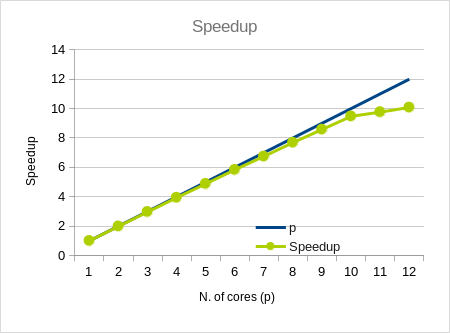
\includegraphics[scale=0.5]{images/omp_speedup.png}
    \caption[]{Lo speedup misurato del programma \textit{omp\_circles} è quasi lineare}
\end{figure}
\begin{figure}[H]
    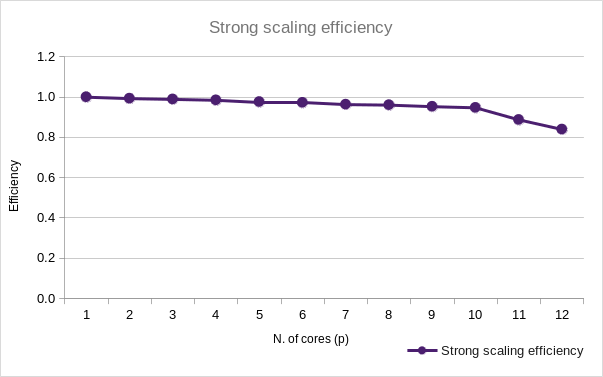
\includegraphics[scale=0.5]{images/omp_strong.png}
    \caption[]{La strong scaling efficiency rimane vicina a 1 con numero di thread minore o uguale a 10 per poi diminuire leggermente}
\end{figure}
La ragione per cui lo speedup diminuisce nella dodicesima iterazione è che il thread probabilmente viene usato dal sistema operativo.
Dato che il carico è bilanciato dinamicamente, ogni thread prende una frazione del lavoro uguale agli altri,
e le prestazioni in weak scaling sono molto buone.
\begin{figure}[H]
    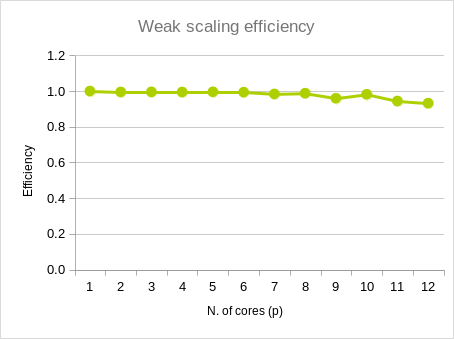
\includegraphics[scale=0.5]{images/omp_weak.png}
    \caption[]{Le prestazioni in weak scaling sono molto buone, rimanendo sempre vicine a 1}
\end{figure}
\section*{Versione MPI}
Usando MPI, dato che ogni processo ha bisogno di ricevere un array aggiornato con tutte le informazioni rilevanti ai cerchi
ho dovuto definire un nuovo data type circle, che ho potuto usare per inviare direttamente le informazioni.
Questo datatype contiene le coordinate x, y, e il raggio r del cerchio. %todo can just send circles once
Questo mi consente di ridurre il numero di MPI\_Bcast necessarie ad ogni iterazione.
Dato che a ogni processo servono le informazioni presenti in tutto l' array, e non solo una porzione, ho usato MPI\_Bcast per facilitare l' invio e non duplicare lavoro,
che sarebbe successo se avessi scelto di usare MPI\_send o  MPI\_recv.
Dopo aver calcolato i nuovi spostamenti sull'asse x e y, ho usato MPI\_reduce.
In questo caso ho preferito codice più semplice al definire una operazione di reduce custom,
che permette efficienza migliore rispetto all' usare direttamente primitive di livello più basso.
Per bilanciare il carico, ho modularizzato il codice e fatto in modo che lo stesso thread che calcola gli spostamenti per il cerchio $i$ lo calcoli anche per il cerchio $n-i$.
Questo risulta nel fatto che a ogni iterazione $i$ del ciclo da $0$ a $\lceil \frac{n}{2} \rceil$, il lavoro fatto rimane costante, dato che il lavoro fatto a ogni iterazione è $i + (n-i) = n$.
Inoltre controllo anche che $n$ sia diverso da $n-i$, per evitare che $n/2$ venga contato due volte nel caso di $n$ dispari.
A questo punto, se un processo itera sullo stesso numero di coppie di cerchi, allora compie lo stesso lavoro di un altro, qualunque sia il suo indice $i$.
Inoltre, ho deciso di usare la funzione reset\_displacement direttamente al posto di mandare il buffer con gli spostamenti resettati a 0.
Questo consente di limitare il numero di comunicazioni tra processi necessarie, e aumenta la porzione di codice parallelizzabile.
Ho anche deciso di mandare i raggi dei cerchi solo una volta, dato che la loro dimensione non cambia.
Questo consente di ridurre la dimensione del payload mandato del 33\%, ma non ho visto notevoli differenze nelle misurazioni.
\begin{figure}[H]
    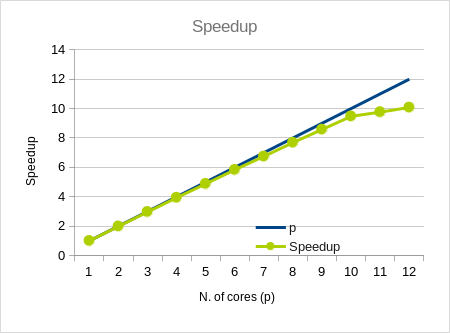
\includegraphics[scale=0.5]{images/mpi_speedup.png}
    \caption[]{Lo speedup rimane molto vicino a lineare con un numero di processi minore o uguale a 10, per poi calare con 11 e 12 processi}
\end{figure}
\begin{figure}[H]
    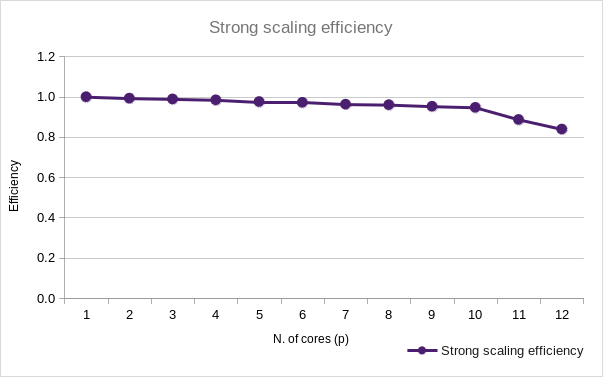
\includegraphics[scale=0.5]{images/mpi_strong.png}
    \caption[short]{La prestazioni in strong scaling rimane vicino a 1 fino a quando si usano 10 processi, e cala fino a 0.8 con 12 processi}
\end{figure}
\begin{figure}[H]
    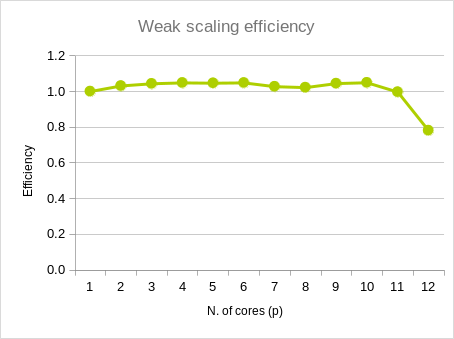
\includegraphics[scale=0.5]{images/mpi_weak.png}
    \caption[short]{La prestazioni in weak scaling rimane vicino a 1 fino a quando si usano 10 processi, e cala fino a 0.8 con 12 processi}
\end{figure}
La ragione per cui lo speedup diminuisce significativamente nella dodicesima iterazione è che il processo probabilmente viene anche usato dal sistema operativo.
\section*{Conclusioni}
Ho ottenuto uno speedup significativo sia nella versione MPI che nella versione OpenMP.
La differenza principale tra il programma MPI e il programma OpenMP è la mancanza di scheduling dinamico nella versione MPI.
Questo è stato risolto bilanciando il carico in modo manuale nella versione MPI, come descritto in precedenza.
Un'altra possibile ottimizzazione è aumentare la cache locality iterando sugli spostamenti x e y separatamente.
Questo consente al programma di dover tenere nella cache solo lo spostamento corrente, effettivamente raddoppiando il numero di spostamenti nella cache.
Ho deciso di non usare questa ottimizzazione, dato che il limite principale del codice OpenMP sembra comunque la comunicazione tra processi.
Ho inoltre notato che il numero di intersezioni non sono esattamente uguali tra versione parallellizzata e seriale, ma differiscono di circa lo 0.5\% alla ventesima iterazione.
Dopo una sessione di debugging, credo che questo sia dovuto al fatto che i float che rappresentano gli spostamenti vengono sommati in un ordine diverso, dando origine così a risultati leggermente inconsistenti.
In conclusione, la versione OpenMP ha risultati migliori leggermente migliore di quella MPI, ma entrambe riescono a ottenere speedup significativi rispetto alla loro corrispettiva versione seriale.
\end{document}
